\documentclass[fontsize=12pt]{scrartcl}
\usepackage[utf8]{vietnam}
\usepackage{amssymb}
\usepackage{amsmath}
\usepackage{algorithm}
\usepackage{url}
\usepackage{subfig}
\usepackage{graphicx}
\usepackage[top=2cm, bottom=3cm, left=3.5cm, right=2cm]{geometry}
\title{Báo cáo đồ án tốt nghiệp}
\renewcommand{\baselinestretch}{1.2}
\setcounter{page}{3}
\usepackage{fancyhdr}
\pagestyle{fancy}
\usepackage{hyperref}
\hypersetup{colorlinks=true,urlcolor=black,linkcolor=black}
\usepackage{changepage}
\usepackage{framed}
\usepackage{multirow}
\usepackage{diagbox}
\usepackage{amsmath}
\usepackage{bm}
\usepackage{listings}
\newcommand{\bigCI}{\mathrel{\text{\scalebox{1.07}{$\perp\mkern-10mu\perp$}}}}

\lhead{}
\chead{}
\rhead{}
\renewcommand{\footrulewidth}{0.4pt}
\lfoot{Sinh viên thực hiện: Vũ Minh Đức - 20131081 Khóa K58 Lớp CNTT2.03}
\cfoot{}
\rfoot{\thepage}

\begin{document}

\newpage
\begin{center}
\textbf{Lời cảm ơn}
\end{center}


\newpage
\begin{abstract}
\begin{center}
\textbf{Tóm tắt đồ án}
\end{center}

\end{abstract}

\newpage
\begin{abstract}
\begin{center}
\textbf{Abstract}
\end{center}
\end{abstract}

\newpage
\tableofcontents

\newpage
\textbf{Danh sách các từ viết tắt và thuật ngữ}
\begin{table}[H]
\begin{center}
\begin{tabular}{|l|l|}
\hline
ANN & Artificial Neural Network\\
\hline
RNN & Recurrent Neural Network\\
\hline
LSTM & Long-Short Term Memory \\
\hline
TDSC & Target-Dependent Sentiment Classification\\
\hline
\end{tabular}
\end{center}
\end{table}


\textbf{Danh sách các kí hiệu dùng trong đồ án}\\
Trong đồ án, các chữ cái thường như H,K,v,w sẽ chỉ các số, các chữ thường được in đâm như $\boldsymbol{v,w,h}$ dùng để chỉ các vector, các chữ viết hoa in đậm để chỉ ma trận như $\boldsymbol{W,Z}$. Ngoài ra còn một số kí hiệu khác như:
\begin{table}[H]
\begin{center}
\begin{tabular}{|l|l|}
\hline
$\cdot$ & dùng để chỉ phép nhân ma trận \\ \hline
$*$ & chỉ phép nhân theo từng thành phần(element-wise multiplication) \\ \hline
$w_c$ & trọng số sử dụng cho bài toán lệch nhãn \\ \hline
\boldsymbol{$W$} & Ma trận trọng số \\ \hline
\boldsymbol{$w_i$} & vector biểu diễn word2vec \\ \hline
\boldsymbol{$h_i$} & vector biểu diễn đầu ra tại tầng ẩn LSTM \\ \hline
\end{tabular}
\end{center}
\end{table}

\newpage
\listoffigures

\newpage
\listoftables
\newpage
%%%%%%%%%%%%%%%%%%%%%%%%%%%%%%%%%%%%%%%%%%%%%%%%%%%%%%%%%%%%%%%%%
\section{Giới thiệu đề tài}
\par
Hiện nay học máy đang được áp dụng rộng rãi trong các ngành công nghiệp và đặc biệt là những bài toán như xử lý ngôn ngữ tự nhiên, xe tự lái, xử lý ảnh. Những hệ thống học máy đã góp phần to lớn trong việc giảm công sức và thời gian làm việc. Việc tạo ra những hệ thống học máy thực hiện tốt các nhiệm vụ trong bài toán xử lý ngôn ngữ tự nhiên là một bài toán quan trọng hỗ trợ máy tính có khả năng tốt trong việc tương tác và xử lý ngôn ngữ mà con người dùng.
\par

Bài toán \textit{phân tích cảm xúc} là một bài toán nhỏ nhưng quan trọng trong lĩnh vực xử lý ngôn ngữ tự nhiên đối với cả tiếng Việt nói chung và các ngôn ngữ khác trên thế giới. Hiện tại bài toán \textit{phân tích cảm xúc} là một bài toán khó bởi những khó khăn chung trong xử lý ngôn ngữ tự nhiên như sai chính tả, tính đa nghĩa, bên cạnh đó cũng có những khó khăn riêng trong bài toán \textit{phân tích cảm xúc} đó là quan điểm cảm xúc thay đổi trong các hoàn cảnh khác nhau, góc nhìn sẽ thay đổi theo cá nhân, theo tâm trạng. Do đó việc tạo ra bộ dữ liệu chuẩn và đồng bộ cũng như xây dựng hệ thống học máy giải quyết bài toán phân tích cảm xúc trở lên rất khó khăn.
\par

Học sâu (Deep learning - DL) là một phần trong lĩnh vực học máy và đang mang lại rất nhiều cảm hứng cũng như tạo ra độ chính xác tốt cho một số bài toán xử lý ảnh, xử lý ngôn ngữ tự nhiên. Những mô hình học sâu dưa trên ý tưởng trừu tượng hóa dữ liệu bằng cách sử dụng các tầng ẩn với các biến đổi phi tuyến. Đặc biệt mô hình Recurrent Neural Network (RNN) rất phù hợp với các bài toán trong xử lý ngôn ngữ tự nhiên.

\par

Đồ án thực hiện cài đặt và thử nghiệm phương pháp học sâu cho bài toán Target-Dependent Sentiment Classification(TDSC), nhiệm vụ của bài toán là với một câu đầu vào và một từ truy vấn cần xác định quan điểm cảm xúc của từ đó tỏng câu là tích cực, tiêu cực, hay trung lập. Những từ truy vấn sẽ là các đối tượng và các thuộc tính của đối tượng.
\par 

Bố cục các phần tiếp theo của đồ án như sau: Phần tiếp theo, phần \ref{sec:intro} sẽ giới thiệu kĩ lưỡng thế nào là mô hình hóa chủ đề, tác dụng của nó, những khó khăn gặp phải với short-text và một số hướng tiếp cận để giải quyết vấn đề với short-text. Phần \ref{sec:basic} sẽ trình bày một số cơ sở lý thuyết về xác suất và đồ thị xác suất sẽ được sử dụng trong đồ án. Thuật toán Expectation-Maximization (EM) \cite{dempster1977maximum} tổng quát ở cả dạng batch và online cũng sẽ được trình bày trong phần này. Tiếp đó, phần \ref{sec:biterm} sẽ giới thiệu mô hình Biterm. Thuật toán học online cho mô hình Biterm sẽ được trình bày trong phần \ref{EMforBTM}. Phần \ref{sec:exp} sẽ trình bày thử nghiệm về hiệu quả của phương pháp được đề xuất cả về thời gian chạy lẫn chất lượng mô hình học được. Cuối cùng, kết luận sẽ được đưa ra ở phần \ref{sec:end}.
\newpage
%%%%%%%%%%%%%%%%%%%%%%%%%%%%%%%%%%%%%%%%%%%%%%%%%%%%%%%%%%%%%%%%%

%%%%%%%%%%%%%%%%%%%%%%%%%%%%%%%%%%%%%%%%%%%%%%%%%%%%%%%%%%%%%%%%%%%%%%%%%%%%%
\section{Cơ sở lý thuyết}\label{sec:basic}
Trong phần này sẽ đưa ra các kiến thức cơ bản về các phương pháp được sử dụng trong bài toán, đồng thời trình bày những bài toán trong phân tích quan điểm.
\subsection{Học máy\textsuperscript{\cite{ wiki:machine_learning}}}
Học máy là một lĩnh vực trong ngành khoa học máy tính, nhằm giúp cho máy tính có khả năng tự học từ dữ liệu để có khả năng giải quyết một vấn đề cụ thể nào đó.
\par
Có thể hiểu rằng học máy là giải quyết một nhiệm vụ T nào đó dựa trên dữ liệu hay những thực nghiệm E và để đo đạc khả năng việc tự học thì ta dùng một độ đo P nào đó để đánh giá xem hệ thống có tự hoạt động tốt hay không. Các thuật toán hay mô hình thực hiện nhiệm vụ học máy được gọi chung là mô hình học máy hay mô hình học.
\par
Một số loại nhiệm vụ T trong học máy mà ta có thể kể đến như sau:
\begin{itemize}
\item Học có giám sát: với nhiệm vụ này, mô hình học được cho đầu vào và giá trị mong muốn ở đầu ra, và nhiệm vụ của mô hình học là học ra cách để từ một đầu vào có thể đưa ra đầu ra tốt nhất. Trong một số trường hợp đặc biệt khác như:
\begin{itemize}
\item Học bán giám sát: dữ liệu đầu ra chỉ có một phần và đa số bị khuyết hay thiếu đầu ra
\item Học tăng cường: dữ liệu huấn luyện được chỉ ra như những phản hồi cho mô hình học, nhiệm vụ này thường thấy trong bài toán xe tự lái, hay trò chơi
\end{itemize}
\item Học không giám sát: mô hình học không được đưa đầu ra mong muốn mà nó cần học ra những cấu trúc bên trong của dữ liệu
\end{itemize}
Ngoài ra dựa vào đầu ra của hệ thống học máy ta có thể phân loại các nhiệm vụ T vào các lớp chính sau:
\begin{itemize}
\item Bài toán phân lớp: với mỗi đầu vào hệ thống sẽ phân vào hai hoặc một vài lớp nào đã được định nghĩa trước. Bài toán này thuộc lớp bài toán học có giám sát.
\item Bài toán hồi quy: là một lớp bài toán học có giám sát nhưng đầu ra là giá trị liên tục thay vì rời rạc như bài toán phân lớp
\item Bài toán phân cụm: hệ thống cần phân dữ liệu vào những cụm mà nó tin ra các dữ liệu trong các cụm cùng tính chất nào đó, đặc biệt các cụm không được định nghĩa trước và thuộc lớp bài toán học không giám sát
\end{itemize}
Trong giới hạn đồ án các kiến thức phía dưới tôi trình bày chủ yếu sẽ tập trung vào bài toán học có giám sát và đặc biệt là bài toán phân lớp.
\subsection{Mạng Neural nhân tạo}\label{subsec:basic_neural}
Mạng neural nhân tạo là một mô hình hay một thuật toán được đưa ra để giải quyết một lớp bài toán trong học máy.
\par
Mạng neuron nhân tạo về cơ bản được mô hình hóa và lấy cảm hứng từ hoạt động của hệ thống thần kinh sinh học. Đồng thời mô hình cũng đạt được nhiều kết quả tốt với các bài toán trong lĩnh vực trí tuệ nhân tạo như xử lý ảnh, xử lý ngôn ngữ, xe tự lái.
\subsubsection{Kiến trúc cơ bản của một neuron cơ bản\textsuperscript{\cite{khoattq}}}\label{subsubsec:basic_neuron}
Mạng neural bao gồm nhiều neuron liên kết và hợp tác để cùng xử lý thông tin. Mạng neural nhân tạo có thể hiểu như là một đồ thị có hướng với các neuron là các nút và các cạnh có hướng cùng với trọng số là các liên kết giữa các đầu vào và đầu ra của các neuron. Hình ảnh minh họa về mạng neural nhân tạo được minh họa như hình \ref{}.\\
Mạng neural nhân tạo nhận đầu vào từ bên ngoài với định dạng dưới dạng các vector. Trọng số này sẽ được nhiều neuron cùng xử lý một lúc. Mỗi neuron sẽ có bộ trọng số riêng. Trong mỗi neuron quá trình tính toán khi nhận được vector đầu vào được mô tả như hình \ref{fig:neuron}. 
\begin{figure*}
     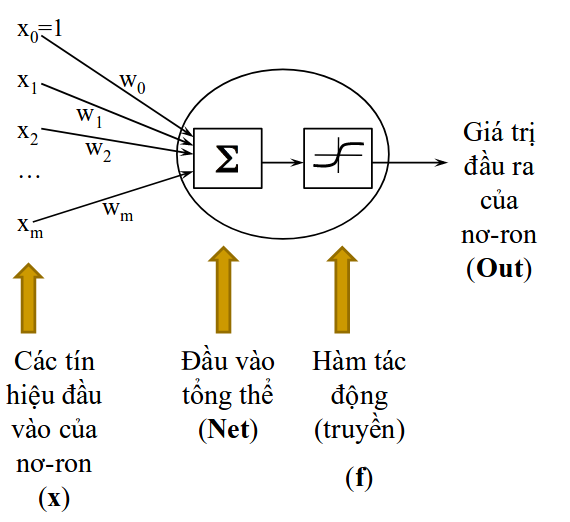
\includegraphics[width=\textwidth]{img/neuron}
      \caption{Cấu trúc hoạt động của một neuron}
       \label{fig:neuron}
\end{figure*}
Dưới đây là mô tả về cách thức hoạt động và những phần tử cơ bản bên trong một neuron. Tại một neuron khi nhận được vector đầu vào, mỗi giá trị đầu vào sẽ gắn với một trọng số tương ứng. Sau đó một đầu vào tổng thể sẽ được tính dựa trên đầu vào và trọng số. Phép tính thường được dùng để tạo ra đầu vào tổng thể là phép cộng.
\begin{align}
Net(\boldsymbol{x},\boldsymbol{w}) = w_0 + w_1x_1 + w_2x_2 + . . . + w_nx_n
\end{align}
Trong đó $w_0$ được coi như trọng số điều chỉnh giúp tạo ra một đầu vào tổng thể  $Net$ được tổng quát hơn. Đầu vào tổng thể sau đó sẽ được dùng để làm đầu vào cho \textit{hàm tác động} và giá trị đầu ra của neuron đó:
\begin{center}
\begin{align}
out = f(Net(\boldsymbol{x},\boldsymbol{w}))
\end{align}
\end{center}
Giá trị đầu ra của một neuron sau đó có thể làm đầu vào cho một neuron khác hoặc dùng để tính giá trị đầu ra.
\subsubsection{Hàm Tác Động\textsuperscript{\cite{khoattq,activation_medium}}}
Như đã nói ở phần \ref{subsubsec:basic_neuron}, mỗi neuron sẽ sử dụng một hàm tác động để tính giá trị đầu ra, dưới đây là một số hàm tác động thường được sử dụng:
\paragraph*{Threshold function}: đối với hàm này giá trị đầu ra sẽ là 0 hoặc 1 dựa vào ngưỡng $\theta$ chọn trước.
\begin{align}
out = TF(Net) = \begin{cases}
                  1, if Net \ge\theta\\
                  0, otherwise
    			\end{cases}
\end{align}
Hàm này tuy đơn giản nhưng lại gặp phải một nhược đểm rất lớn đó là không liên tục, do đó việc sử dụng các thuật toán tối ưu sẽ rất khó khăn.
\paragraph*{Linear function}: hàm này thực hiện một biến đổi tuyến tính giá trị tổng hợp đầu vào:
\begin{align}
out = TF(Net) = \begin{cases}
                  \alpha Net,
    			\end{cases}
\end{align}
Mặc dù hàm liên tục và có đạo hàm nhưng có một điều làm hàm biến đổi tuyến tính không được sử dụng nhiều đó là bởi vì đạo hàm của hàm tuyến tính này với mọi giá trị dù giá trị $Net$ nhỏ hay lớn thì đều giống nhau và là một hằng số. Do đó hàm số này có đạo hàm không phụ thuộc vào đầu vào nên sẽ không phản ảnh được mức độ quan trọng khác nhau của từng đâu vào khi ta sử dụng đạo hàm để cập nhập các tham số như mô tả ở phần \ref{otp:gradient}. Và nếu chỉ dùng hàm tuyến tính thì toàn bộ neuron cuối cùng sẽ chỉ là những biến đổi tuyến tính sẽ không phù hợp với trường hợp dữ liệu phức tạp như trường hợp bài toán phân loại dữ liệu không phân tách tuyến tính.
\paragraph*{Sigmoid function}: giá trị đầu ra sẽ là một số liên tục nằm giữa 0 và 1, hàm được tính theo công thức sau:
\begin{align}
out = Sg(Net) = \begin{cases}
                  \frac{1}{1+e^{-Net}},
    			\end{cases}
\end{align}
Như minh họa ở hình \ref{fig:sigmoid} thì hàm sẽ tiến rất nhanh về giá trị 1 và -1 và bão hòa khi giá trị đầu vào $Net$ lớn hơn 6 hoặc nhỏ hơn -6. Do đó hàm \textit{sigmoid} dù có ưu điểm nhưng không được sử dụng nhiều đặc biệt là với các mạng neural nhân  tạo có nhiều neuron được chồng thành nhiều tầng.
\begin{figure*}
     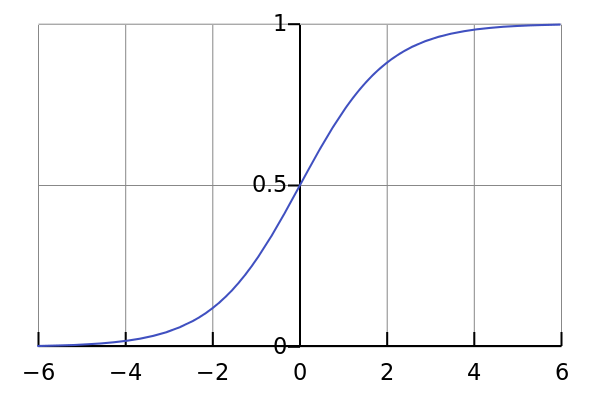
\includegraphics[width=\textwidth]{img/sigmoid_}
      \caption{Hàm sigmoid}
       \label{fig:sigmoid}
\end{figure*}
\paragraph*{ReLu function}: là một hàm kết hợp giữa hàm ngưỡng và hàm tuyến tính, được tính theo công thức sau:
\begin{align}
out = ReLu(Net) = max(0,Net)
\end{align}
Với trường hợp đầu vào là lớn hơn 0 thì hàm \textit{ReLu} cũng giống như hàm \textit{Linear function}, và như thế với những trường hợp mà đầu vào lớn hơn 0 thì chúng đều được cập nhập giống nhau. Tuy nhiên hàm \textsc{ReLu} có những ưu điểm khác làm nó được sử dụng. Nó không phải hàm tuyến tính như mô tả ở trên nên có thể sử dụng để ước lượng các trường hợp để ước lượng một phàm phi tuyến tổng quát. Ngoài ra việc tính toán khi sử dụng hàm \textit{ReLu} cũng trở lên đơn giản và đỡ tốn kém.
\subsubsection{Hàm lỗi và hàm mục tiêu}
Trong giới hạn đồ án tôi xin chỉ đưa ra hàm lỗi với trường hợp học có giám sát.
\par
Với bài toán học có giám sát, khi một mô hình hình học nhận đầu vào là vector $\boldsymbol{x}$ và dự đoán đầu ra là $\boldsymbol{y}'$, trong khi đó đầu ra mong muốn của chúng ta là $\boldsymbol{y}$. Lúc này hàm lỗi là hàm chỉ ra mức độ phạt mà mô hình phải chịu, kí hiệu tổng quát cho hàm lỗi với đầu vào $\boldsymbol{x}$, giá trị đầu ra mong muốn $\boldsymbol{y}$, và các tham số hô hình cần học là $\boldsymbol{W}$: $L(\boldsymbol{x}, \boldsymbol{y}, \boldsymbol{W})$.
\par
Với một mô hình học ta muốn mô hình đạt khả năng tốt nhất có thể, nên mục tiêu của việc huấn luyện mô hình học máy là tìm mô hình sao cho dự đoán tốt nhất có thể, hay nói cách khác là ít lỗi nhất. Từ đó ta có định nghĩa hàm mục tiêu như sau:
\begin{align}
\boldsymbol{W}^* = \displaystyle\min_{\boldsymbol{W}}L_{\boldsymbol{x}, \boldsymbol{y}\in P(data)}(\boldsymbol{x}, \boldsymbol{y}, \boldsymbol{W})
\end{align}
Trong đó P(data) là phân phối của dữ liệu và $\boldsymbol{x}, \boldsymbol{y}$ là toàn bộ dữ liệu thuộc phân phối đó.
\par
Tuy nhiên trên thực tế thì ta hoàn toàn không biết được phân phối của dữ liệu là gì và ta chỉ có một tập nhỏ quan sát được, gọi là tập huấn luyện hay kí hiệu là $\boldsymbol{D}$. Và do đó ta chỉ có thể ước lượng giá trị hàm mục tiêu trên tập thực nghiệm này với mong muốn mô hình hoạt động tốt trên $\boldsymbol{D}$. Do đó hàm mục tiêu được viết lại thành:
\begin{align}
\boldsymbol{W}^* = \displaystyle\min_{\boldsymbol{W}}L_{\boldsymbol{x}, \boldsymbol{y}\in \boldsymbol{D}}(\boldsymbol{x}, \boldsymbol{y}, \boldsymbol{W})
\end{align}
Tùy vào bài toán mà hàm lỗi và hàm mục tiêu thích hợp sẽ được sử dụng. Dưới đây tôi xin trình bày về hàm lỗi và hàm mục tiêu thường hay được sử dụng cho bài toán phân loại, đặc biệt là với các bài toán phân loại sử dụng mô hình học sâu.
\par
Với bài toán phân loại, dạng đầu ra thường được sử dụng trong học sâu là thể hiện xác suất ứng với từng nhãn lớp mà mô hình nghĩ nó có khả năng thuộc vào. Giả sử bài toán ta cần thực hiện phân loại vào K lớp, thì với một đầu vào, mô hình sẽ đưa ra dự đoán là một vector $\boldsymbol{p}$ với $p_i$ thể hiện xác suất rằng dữ liệu đầu vào sẽ thuộc lớp i, $\boldsymbol{p}$ là vector K phần tử.
\par
Do là bài tóan học có giám sát nên ta sẽ biết rằng với một đầu vào thì nó sẽ thuộc vào lớp nào. Do đó ta có thể coi đầu ra là một vector $\boldsymbol{q}$ K chiều với phần tử thứ j bằng 1 thể hiện lớp của dữ liệu đầu vào và các phần tử khác bằng 0. Trong trường hợp này mô hình tốt thì hai phân phối xác suất ứng với $\boldsymbol{p}, \boldsymbol{q}$ sẽ gần nhau hoặc giống nhau nhất có thể. Từ đó hàm \textit{cross-entropy} sử dụng để đo mức độ khác nhau giữa hai phân phối xác suất ứng với $\boldsymbol{p}$ và $\boldsymbol{q}$:
\begin{align}
H(p,q) = -\displaystyle\sum_{\boldsymbol{x}, \boldsymbol{y}\in \boldsymbol{D}}\sum_{K}p_i(\boldsymbol{x}, \boldsymbol{y},\boldsymbol{W})\log q_i
\end{align}
Hàm mục tiêu lúc đó sẽ là
\begin{align}
H(p,q) = \displaystyle\min_{\boldsymbol{W}}H(p,q)
\end{align}
Ngoài những mô tả ở trên là học tham số của mô hình thì ngoài ra ta có thể học kiến trúc mô hình. Tuy nhiên trong giới hạn đồ án tôi không trình bày phần này.
\subsubsection{Các kiến trúc mạng neural\textsuperscript{\cite{khoattq}}}
Một mạng neural nhân tạo sẽ gồm có:
\begin{itemize}
\item một tầng đầu vào
\item một tầng đầu ra
\item một hoặc nhiều tầng ẩn được tạo bởi các neuron, là các tầng nằm giữa tầng đầu vào và tầng đầu ra
\end{itemize}
\begin{figure*}
     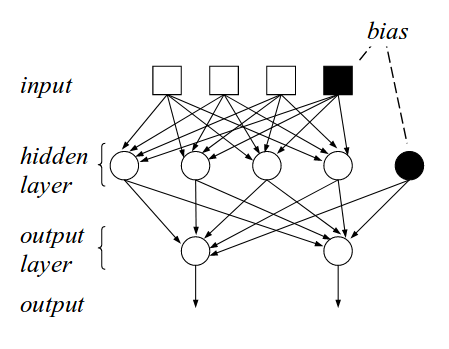
\includegraphics[width=\textwidth]{img/neural_sample}
      \caption{Minh họa một mạng neural nhân tạo}
       \label{fig:neural_sample}
\end{figure*}
Kiến trúc của một mạng neural nhân tạo được xác định bởi:
\begin{itemize}
\item Số lượng các tín hiệu đầu vào
\item Số lượng các tầng
\item Số lượng neuron trong mỗi tầng
\item Số lượng các trọng số của neuron
\item Cách thức các neuron liên kết với nhau trong một tầng hoặc giữa các tầng với nhau
\item Những neuron nào nhận tín hiệu điều chỉnh lỗi
\end{itemize}
Một mạng neural nhân tạo được gọi là liên kết đầy đủ (fully connected) nếu mọi đầu ra từ một tầng liên kết trực tiếp với neuron tầng kế tiếp nó.
Mạng neural nhân tạo có hai kiểu kiến trúc chính như sau:
\begin{itemize}
\item Mạng lan truyền tiến: là mạng mà đầu ra của một tầng chỉ liên kết với neuron của tầng kế tiếp và không có liên kết với các neuron cùng tầng hay tầng trước đó. Minh họa ở hình \ref{fig:feedforward_nn}
\item Mạng phản hồi: trái lại với mạng lan truyền tiến, trong mạng phản hồi đầu ra của một neuron sẽ làm đầu vào(liên kết với) neuron ở cùng tầng hoặc tầng trước nó. Minh họa ở hình \ref{fig:phan_hoi}. Các mạng phản hồi tạo thành các vòng lặp kín được gọi là mạng hồi quy(Reccurent neural network) sau sẽ được viết tắt là RNN. Minh học mô hình hồi quy như hình \ref{fig:rnn_form}
\end{itemize}
\begin{figure*}
     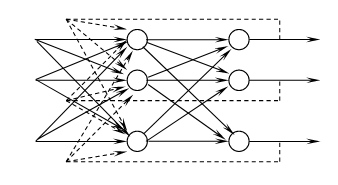
\includegraphics[width=\textwidth]{img/feedforward_nn.png}
      \caption{Minh họa mạng lan truyền tiến}
       \label{fig:feedforward_nn}
\end{figure*}
\begin{figure*}
     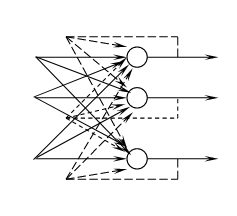
\includegraphics[width=\textwidth]{img/hoi_quy}
      \caption{Minh họa mạng phản hồi}
       \label{fig:phan_hoi}
\end{figure*}
\begin{figure*}
     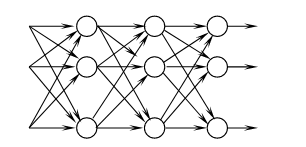
\includegraphics[width=\textwidth]{img/rnn_form}
      \caption{Minh họa mạng hồi quy}
       \label{fig:rnn_form}
\end{figure*}
\subsection{Thuật toán học\textsuperscript{\cite{Goodfellow-et-al-2016,khoattq}}}
Có hai kiểu học chính được sử dụng trong mạng neural nhân tạo là học tham số và học cấu trúc mạng.
\begin{itemize}
\item Học tham số: mục tiêu là thay đổi các trọng số trong mạng
\item Học cấu trúc: mục tiêu là học và thay đổi thích nghi cấu trúc mạng bao gồm số lượng neuron và cách thức liên kết giữa các neuron.
\end{itemize}
Trong đồ án tôi chỉ xét trường hợp học tham số.
\par
Các thuật toán học sâu hầu hết sẽ đều đưa về việc tối ưu hóa một hàm số nào đó. Việc tối ưu hóa hoặc là đi tìm giá trị nhỏ nhất hoặc là đi tìm giá trị lớn nhất của hàm số $f(x)$ bằng cách thay đổi giá trị của $x$. Chúng ta hoàn toàn có thể coi bài toán tối ưu là đi tìm giá trị nhỏ nhất của  $f(x)$. Đối với bài toán tìm giá trị lớn nhất cho hàm số $f(x)$ ta có thể chuyển về bài toán tìm giá trị nhỏ nhất của hàm số $-f(x)$.
\paragraph*{Tối ưu dựa vào Gradient}\label{opt:gradient}:
\par
Hàm số mà ta muốn đi tìm giá trị nhỏ nhất hoặc lớn nhất gọi là hàm mục tiêu hay có thể gọi là hàm lỗi. Đặt giá trị của $x$ tại đó hàm số đạt giá trị lớn nhất hoặc nhỏ nhất là $x^*$.
Đạo hàm của hàm số $f(x)$ được kí hiệu là $f'(x)$. Vi phân của một hàm số sẽ cho ta giá trị về độ dốc của hàm số tại điểm $f(x)$ đang được xét. Hay nói cách khác nó sẽ chỉ ra rằng mức độ thay đổi của $f(x)$ khi ta thay đổi một lượng nhỏ quanh giá trị $x$ : $f(x+\epsilon) = f(x) + \cdot f'(x)$
\par
Do đó mà giá trị của đạo hàm sẽ chứa thông tin hữu ích cho việc đi cực tiểu hóa một hàm số bởi vì nó sẽ cho ta biết rằng thay đổi $x$ như thế nào để nhận được một giá trị nhỏ hơn cho $f(x)$. 
\par
Khi giá trị đạo hàm bằng 0, nó sẽ không cung cấp cho chúng ta thông tin về hướng dịch chuyển để cực tiểu hóa hàm mục tiêu. Những điểm như thế ta coi nó là điểm cực trị. Một điểm gọi là điểm cực tiểu nếu giá trị của nó nhỏ hơn so với các điểm lân cận của nó. Một điểm là cực đại nếu giá trị của nó là lớn hơn so với các điểm lân cận của nó. Trong một số trường hợp điểm cực trị nhưng không phải là điểm cực tiểu và cực đại thì nó sẽ là điểm yên ngựa. Minh họa các kiểu điểm cực trị được mô tả ở hình \ref{fig:critical_point} .
\begin{figure*}
     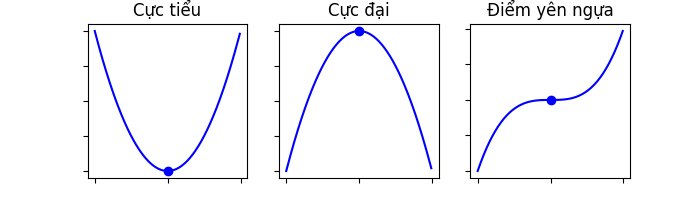
\includegraphics[width=\textwidth, scale = 0.1]{img/critical_point}
      \caption{Các điểm cực trị}
       \label{fig:critical_point}
\end{figure*}
\par
Điểm mà tại đó hàm số đạt giá trị nhỏ nhất được gọi là điểm cực tiểu toàn cục. Một hàm số thì có thể có một vài điểm cực tiểu hay cực đại địa phương. Trong tối ưu hóa hàm lỗi cho mô hình học sâu, hàm lỗi có rất nhiều điểm cực tiểu địa phương và điểm yên ngựa. 
\par
Chúng ta thường đi tối ưu một hàm số mà đầu vào có n chiều và đầu ra là một chiều: $f: \boldsymbol{\mathbb{R}^n}\Rightarrow \mathbb{R}$.
\par
Đối với những hàm số đầu vào là nhiều chiều, chúng ta sử dụng đạo hàm thành phần. Đạo hàm thành phần là đạo hàm được tính cho một chiều $x_i$ đầu vào. Đạo hàm thành phần theo chiều $x_i$ được kí hiệu là $\frac{\delta}{\delta x_i}f(\boldsymbol{x})$, giá trị này sẽ mô tả việc thay đổi giá trị của $x_i$ tại lân cận của $x_i$ sẽ ảnh hưởng ít hay nhiều đến giá trị của hàm $f$. Khi này đạo hàm của hàm f sẽ là một vector bao gồm tất cả các đạo hàm thành phần và được kí hiệu là $\Delta_{\boldsymbol{x}}f(\boldsymbol{x})$. Khi này điểm cực trị của hàm số là điểm mà tạo đó tất cả các đạo hàm thành phần băng 0.
\par
Đạo hàm của hàm $f$ theo hướng $\boldsymbol{u}$ là giá trị thể hiện mức độ thay đổi của hàm $f$ tại vị trí $\boldsymbol{x}$ theo hướng $\boldsymbol{u}$ với $\boldsymbol{u}$ là vector đơn vị.
Đạo hàm có hướng được tính theo định nghĩa như sau:\\
\begin{center}
$\Delta_{\boldsymbol{u}} f = \lim\limits_{\alpha\rightarrow 0}\frac{f(\boldsymbol{x}+\alpha \boldsymbol{u}) - f(\boldsymbol{x})}{\alpha}$
\end{center}
\par
Từ định nghĩa này ta có phép biến đổi sau:
 
\begin{center}
$\Delta_{\boldsymbol{u}} f = \boldsymbol{u^T} \lim\limits_{\alpha\boldsymbol{u}\rightarrow 0}\frac{f(\boldsymbol{x}+\alpha \boldsymbol{u}) - f(\boldsymbol{x})}{\alpha\boldsymbol{u}}$
\end{center}
Có được biến đổi trên là bởi vì $\boldsymbol{u}$ là một vector đơn vị, và là một hằng số, do đó khi $\alpha$ tiến tới 0 cũng tương đương với $\alpha u_i$ tiến tới 0 với $u_i$ là phần tử thứ i của vector u. Đồng thời $\lim\limits_{\alpha\boldsymbol{u}\rightarrow 0}$ được hiểu là giới hạn theo từng chiều, nếu đặt:
\begin{center}
$\boldsymbol{l} =  \lim\limits_{\alpha\boldsymbol{u}\rightarrow 0}\frac{f(\boldsymbol{x}+\alpha \boldsymbol{u}) - f(\boldsymbol{x})}{\alpha\boldsymbol{u}}$
\end{center}
Thì phần tử thứ i trong vector $\boldsymbol{l}$ được hiểu như sau:
\begin{center}
$l_i = \lim\limits_{\alpha\ u_i\rightarrow 0}\frac{f(x_i+\alpha u_i) - f(x_i)}{\alpha u_i}$
\end{center}
Do đó ta có thể viết lại công thức đạo hàm theo hướng u dưới công thức sau: 
\begin{center}
$\frac{\delta}{\delta\alpha}f(\boldsymbol{x}+\alpha \boldsymbol{u}) = \boldsymbol{u}^T\cdot\Delta_{\boldsymbol{x}}f(\boldsymbol{x})$
\end{center}
\par
Để tìm giá trị cực tiểu cho hàm số $f$, trong bài toán học sâu với dữ liệu nhiều thì ta sử dụng cách tiếp cận, mỗi một bước học ta sẽ tìm đến một giá trị nhỏ hơn giá trị hiện tại. Với ý tưởng đó, thì ta cần tìm hướng mà tại đó giá trị của hàm $f$ giảm nhanh nhất. Và từ định nghĩa đạo hàm theo hướng của hàm số  ta có thể ứng dụng để tìm hướng tốt nhất để giảm hàm mục tiêu. Nhận thấy rằng nếu hướng theo vector $\boldsymbol{u}$ làm giảm giá trị của hàm $f$ thì giá trị của đạo hàm theo hướng $\boldsymbol{u}$ sẽ mang giá trị âm, trái lại sẽ mang giá trị dương. Như thế ta thấy hướng làm giảm giá trị hàm $f$ nhiều nhất sẽ được tìm theo:
\begin{center}
\begin{align}\label{formulation:cthuc}
\min_{\boldsymbol{u}}\boldsymbol{u}^T\cdot\Delta_{\boldsymbol{x}}f(\boldsymbol{x})
 = \displaystyle\min_{\boldsymbol{u}}\Vert\boldsymbol{u}\Vert_2\Vert\Delta_{\boldsymbol{x}}f(\boldsymbol{x})\Vert_2\cos(\theta)\end{align}
\end{center}
Với $\theta$ là góc giữa vector $\boldsymbol{u}$ và vector đạo hàm của f. Ta thấy rằng $\Vert\boldsymbol{u}\Vert_2 = 1$, và  $\Vert\Delta_{\boldsymbol{x}}f(\boldsymbol{x})\Vert_2$ không phụ thuộc vào $\boldsymbol{u}$ nên ta có thể thấy rằng biểu thức \ref{formulation:cthuc} tương đương với: $\min_{\boldsymbol{u}}\cos(\theta)$. Biểu thức này đạt giá trị nhỏ nhất là -1 khi $\theta=\pi$ hay vector $\boldsymbol{u}$ ngược hướng với hướng của vector đạo hàm. Từ chứng minh trên ta có thể kết luận rằng với các hàm số tồn tại đạo hàm, nếu di chuyển một điểm xung quanh lân cận của nó theo hướng đạo hàm thì sẽ làm tăng giá trị hàm số nhanh nhất và di chuyển theo hướng ngược đạo hàm sẽ làm hàm số giảm nhanh nhất. Do đó để giảm giá trị của hàm $f$ ta di chuyển theo hướng ngược với hướng đạo hàm, và phương pháp sử dụng ý tưởng này gọi là \textit{gradient descent}. Công thức tìm điểm dịch chuyển mới theo phương pháp được  thể hiện như sau:
\begin{align}
\boldsymbol{x'} = \boldsymbol{x} - \epsilon\Delta_{\boldsymbol{x}}f(\boldsymbol{x})
\end{align}
Trong đó $\epsilon$ được gọi là tốc độ học, nó quyết định độ lớn của bước nhảy. Có một số cách để lựa chọn tốc độ học, một cách thường được áp dụng là lựa chọn $\epsilon$ là một hằng số có giá trị đủ nhỏ.
\par
Ngoài ra bên cạnh việc ứng dụng giá trị đạo hàm cấp 1 để tối ưu hàm số $f$ thì ta có thể dùng thêm thông tin về đạo hàm cấp 2. Trong giới hạn của đồ án thì phần này tôi xin phép không đi sâu vào.
\paragraph*{Một số phương pháp cơ bản dựa vào Gradient}:\\
Như đã giới thiệu ở mục \ref{opt:gradient}, thì học dựa trên đạo hàm, hay phương pháp \textit{gradient descent} là phương pháp học dựa vào đạo hàm trên toàn bộ tập huấn luyện. Tuy nhiên với trường hợp dữ liệu rất nhiều thì cách này trở nên bất tiện bởi số lượng tính toán các phép tính. Do đó phương pháp \textit{stochastic gradient descent} là một phương pháp dựa trên ý tưởng của \textit{gradient descent} nhưng thay vì sử dụng toàn bộ dữ liệu huấn luyện thì chỉ lấy ngẫu nhiên một số lượng nhỏ dữ liệu đưa vào để tính và ước lượng giá trị của đạo hàm và thay đổi các tham số dựa trên đạo hàm được ước lượng đó. Phương pháp \textit{stochastic gradient descent} được mô tả ở thuật toán 1
\begin{table}[ht]
\begin{center}
  \begin{tabular}{l}
\hline
Thuân toán 1: \textit{stochastic  gradient descent}\\
\hline
Đầu vào : tốc độ học $\epsilon$, các tham số khởi tạo $\theta$\\
while (chưa đạt tiêu chí dừng) do:\\
\hspace{1em} lấy ngẫu nhiên m dữ liệu từ tập huấn luyện \{$\boldsymbol{x}^{(1)}, \boldsymbol{x}^{(2)}, . . , \boldsymbol{x}^{(m)}$\} cùng với nhãn tương ứng $y_{(i)}$\\
end while\\
  \end{tabular}
  \end{center}
\end{table}%
\paragraph*{Phương pháp kết hợp với tốc độ học}
\paragraph*{Lựa chọn phương pháp tối ưu phù hợp}
\subsection{Thuật toán lan truyền ngược}
giới thiệu về thuật toán lan truyền ngược
\subsection{Mô hình Recurrent Neural Network và Long-Short Term Memory}
\par
Giới thuệu về mô hình RNN
\subsection{Vấn đề overfit và cách giải quyết}
Giới thiệu định nghĩa overfit và các cách thường dùng để giải quyết: dropout, weight decay, . .. 
%%%%%%%%%%%%%%%%%%%%%%%%%%%%%%%%%%%%%%%%%
\subsection{Bài toán xử lý ngôn ngữ tự nhiên và phân tích quan điểm Target-Dependent Sentiment Classification}
\par
Bài toán xử lý ngôn ngữ tự nhiên là một nhánh trong lĩnh vực khoa học máy tính và trí tuệ nhân tạo liên quan đến việc tương tác giữa máy tính và ngôn ngữ tự nhiên mà con người sử dụng. Việc máy tính có thể hiểu tốt được ngôn ngữ tự nhiên sẽ giúp ích rất nhiều cho việc phát triển của nhân loại. Nếu hiểu được ngôn ngữ của con người thì máy tính có thể thực hiện và giải quyết một lượng lớn công việc khó khăn và nhàn chán thay con người như: dịch thuật, tìm kiếm thông tin, tóm tắt văn bản, hoặc có thể tương tác trực tiếp với con người qua ngôn ngữ tự nhiên và hỗ trợ như một trợ lý ảo, như một người tư vấn trong công việc, đời sống và sức khỏe. Một số bì toán chính trong xử lý ngôn ngữ tự nhiên có thể kể đến như:
\begin{itemize}
\item Bài toán phân tích cú pháp: là những lớp bài toán liên quan đến những pháp như bài toán tách câu, bài toán tách từ, bài toán Part-of-speech tagging
\item Bài toán ngữ nghĩa: là những lớp bài toán phân tích ngữ nghĩa của ngôn ngữ như bài toán phân tích quan điểm, bài toán dịch máy
\item Bài toán phân tích giọng nói: là những lớp bài toán liên quan đến giọng nói như nhận diện giọng nói, hay Text-to-Speech
\end{itemize}
\par
Bài toán phân loại cảm xúc là một bài toán con trong lĩnh vực xử lý ngôn ngữ tự nhiên và hiện tại đang được quan tâm rất nhiều không chỉ trong nghiên cứu mà ngay cả các doanh nghiệp. Bài toán phân tích quan điểm, cảm xúc, thái độ của ai đó về một sự kiện, đối tượng, cá nhân hay các thuộc tính của một đối tượng. Việc phân tích cảm xúc là cực kì quan trọng, đối với cá nhân khi mua sản phẩm họ sẽ tìm hiểu xem các trang báo nói tốt hay xấu về sản phẩm ra sao, người dùng đánh giá như thế nào.  Bên cạnh đó, với những tập đoàn, nhà sản xuất họ cũng muốn đánh giá cộng đồng đánh giá và đang nói gì về mình hay về đối thủ của mình để từ đó đưa ra được những chính sách và cải thiện hoặc đưa ra sản phẩm mới.
Phần này cần trình bày thêm về bài toán sentiment
\newpage
%%%%%%%%%%%%%%%%%%%%%%%%%%%%%%%%%%%%%%
%%%%%%%%%%%%%%%%%%%%%%%%%%%%%%%%%%%%%%%%%%%%%%%%%%%%%%%%%%%%%%%%%%
\section{Ứng dụng học sâu vào bài toán Target-Dependent Sentiment Classificaiton}\label{EMforBTM}
\par
Trong phần này sẽ trình bày phương pháp sử dụng học sâu cho bài toán Target-Dependent Sentiment Classification với bộ dữ liệu được tôi xây dựng với dữ liệu về xe trên ngôn ngữ tiếng Việt được thu thập từ các trang báo mạng.
\subsection{Bài toán Target-Dependent Sentiment Classification}
\par
Bài toán Target-Dependent Sentiment Classification(TDSC)\textsuperscript{\cite{tang2015effective}} là bài toán giải quyết vấn đề với một câu trong văn bản và một từ truy vấn nhiệm vụ là phân loại cảm xúc (tích cực, tiêu cực hay trung lập) của từ truy vấn(sau sẽ gọi tắt là truy vấn) đó theo ngữ cảnh của câu, ví dụ với câu: \textit{đèn pha được thiết kế với choá phản quang ngũ giác , hình dáng như một viên kim cương năm cạnh , làm tăng thêm nét quyến rũ}, nếu từ truy vấn được truyền vào là \textit{đèn pha} thì nhãn quan điểm mong muốn với từ truy vấn này sẽ là \textit{tích cực}. Những từ truy vấn có thể là một thực thể, hay một khía cạnh của thực thể nào đó. Bài toán hiện đang được quan tâm bởi nhiều nhà nghiên cứu và danh nghiệp bởi mức độ khó của bài toán cũng như tính ứng dụng thực tế.
Cần phân tích thêm về lợi ích của bài toán ở phần này
\subsection{Một số phương pháp hiện tại}
Phần này tôi sẽ đi mô tả lại một vài phương pháp đang được sử dụng để giải quyết bài toán Target-Dependent Sentiment Classification
\subsubsection{Phương thức Target-Independent}
Một số cách giải quyết đã được thực hiện trên bộ dữ liệu tiếng anh chỉ đơn giản sử dụng những mô hình phân lớp cho bài toán phân tích quan điểm văn bản. Với Alec Go và cộng sự\textsuperscript{\cite{go2009twitter}} đã sử dụng cách biểu diễn n-gram cho tất cả các từ trong một câu truy vấn, tuy nhiên điều đó là không phù hợp bởi vì rất nhiều trường hợp các từ truy vấn trong một câu nhưng có quan điểm cảm xúc khác nhau, như trường hợp sau: \textit{hàng loạt các ông lớn như toyota , honda , nissan đều suy giảm từ 4-15 $\%$ trong mảng xe phổ thông , riêng mazda tăng trưởng cao nhất thị trường với mức tăng 20$\%$}, thì các từ truy vấn \textit{toyota, honda, nissan} sẽ mang tính chất tiêu cực và trái ngược với \textit{mazda} sẽ mang tính chất tích cực. Như thế nếu chỉ biểu diễn theo cách giải quyết phân loại cho văn bản thì sẽ không thực sự phù hợp với bài toán TDSC.
\subsubsection{Phương thức Target-Dependent}
Thay vì tiếp cận sử dụng phương pháp Target-Independent, phương pháp phân tích dựa trên từ truy vấn sẽ được kì vọng đạt được kết quả tốt hơn. Với ý tưởng đó nhóm tác giả Dong\textsuperscript{\cite{dongadaptive}} đã tiếp cận dựa trên phương pháp học sâu, bằng cách sử dụng kết hợp Recursive Neural Network và bài toán Dependency trong xử lý ngôn ngữ tự nhiên trong học máy. Bên cạnh đó nhóm tác giả Tang\textsuperscript{\cite{tang2015effective}} cũng sử dụng hướng tiếp cận sử dụng học sâu nhưng sử dụng LSTM. Với cách tiếp cận này tác giả đã cải thiện độ chính xác cũng như khai thác được tính liên quan giữa từ truy vấn và ngữ cảnh của câu.
\par
Trong bài báo, tác giả sử dụng mô hình LSTM, mỗi từ đầu vào sẽ được biểu diễn bởi một vector liên tục dựa trên lý thuyết word embedding\textsuperscript{\cite{bengio2003neural}}, một điều cần lưu ý là truy vấn có thể là một từ hoặc một cụm từ như "Honda", "Honda Alpha", . . . Toàn bộ từ được lưu và biểu diễn bởi một vector L$_{w}$ $\in R^{d*V}$, với d là số chiều của vector biểu diễn cho một từ và V là số lượng các từ trong tập từ điển. Ý tưởng cơ bản của bài báo dựa trên quan sát quan điểm mỗi truy vấn sẽ được mô tả bởi các từ phía trước và phía sau xung quanh nó, vì vậy biểu diễn ngữ cảnh của các từ phía trước và phía sau sẽ được sử dụng cho việc phân loại quan điểm cảm xúc cho truy vấn . Do đó tác giả sử dụng hai mô hình LSTM, một mô hình LSTM$_{l}$ sẽ nhằm mục đích biểu diễn ngữ nghĩa cho truy vấn dựa trên các từ bên trái, một mô hình LSTM$_{r}$ sẽ nhằm mục đích biểu diễn nghữ nghĩa cho truy vấn dựa trên các từ bên phải. Minh họa của mô hình được vẽ lại dựa trên ý tưởng của bài báo ở hình [ref]. Trong mô hình đầu vào của mạng LSTM$_{l}$ sẽ gồm có các từ bên trái cùng với các từ trong truy vấn, tương tự như thế đầu vào cho mô hình LSTM$_{r}$ sẽ gồm các từ truy vấn và các từ phía bên phải. Trong báo cáo tác giả đặt tên cho mô hình là Target-Dependent Long Short Term Memory(kí hiệu TD-LSTM), mô hình được minh họa theo hình \ref{img_td_lstm}.
\begin{figure*}
     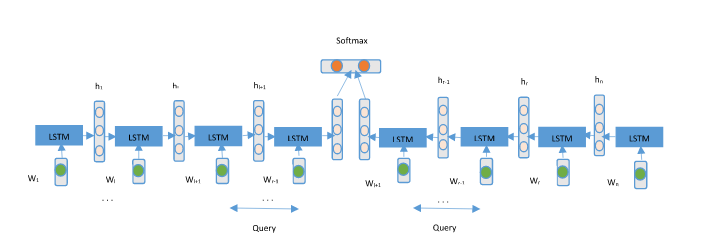
\includegraphics[width=\textwidth]{img/td_lstm}
      \caption{Phương pháp target-connection long short-term memory (TC-LSTM) cho bài toán  target-dependent sentiment classification, . . . . }
       \label{img_td_lstm}
\end{figure*}
\par
Tuy nhiên tác giả giả thuyết rằng mỗi một từ đích thì sẽ có những tương tác với các từ trong câu khác nhau nên cần có biểu diễn để tích hợp từ đích cùng  với các từ trong câu. Để giải quyết tác giả đã biểu diễn truy vấn bởi một vector v$_{target}$ bằng cách cộng tất cả các giá trị của từng từ truy vấn lấy từ mô hình word embedding sau đó lấy trung bình dựa trên số lượng các từ trong từ truy vấn, sau đó biểu diễn v$_{target}$. Sau khi có được biểu diễn cho từ đích này, với mỗi đầu vào cho LSTM$_{l}$ và LSTM$_{r}$ tác giả thực hiện gép vector biểu diễn của từ đầu vào cùng với vector v để tạo thành một vector có số chiều tăng gấp đôi. Mô hình sau khi thêm hiệu chỉnh này được đặt tên là Target-Connection Long Short Term Memory( TC-LSTM), mô hình được minh họa theo hình \ref{img_tc_lstm}.
\begin{figure*}
     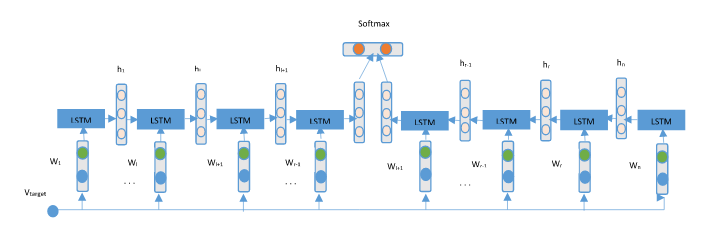
\includegraphics[width=\textwidth]{img/tc_lstm}
      \caption{Phương pháp target-connection long short-term memory (TC-LSTM) cho bài toán  target-dependent sentiment classification, . . . . }
       \label{img_tc_lstm}
\end{figure*}
\par
Cả hai mô hình TD-LSTM và TC-LSTM sau khi qua mạng LSTM$_{l}$ và LSTM$_{r}$, tác giả thực hiện ghép hai giá trị đầu ra ở tẩng ẩn của LSMT$_{l}$ và LSTM$_{r}$ sau đó đưa qua một lớp tuyến tính với số lượng đầu ra sẽ tương ứng với số nhãn cần phân loại trong bài toán phân tích quan điểm.
\begin{center}
$\boldsymbol{logit} = \boldsymbol{W}\cdot[\boldsymbol{h_{l}},\boldsymbol{h_{r}}]$\\
\end{center}

Với $\boldsymbol{W}$ là ma trận Kx2H, K là số đầu ra mong muốn, H là độ dài của vector ở tầng ẩn của LSTM.
\par
Kết quả sau khi qua tầng tuyến tính đưa thêm tầng softmax để biểu diễn dự đoán cho mỗi lớp dưới ý nghĩa xác suất của mỗi nhãn.
\begin{center}
$P_k(q) = \dfrac{exp(logit_i)}{\sum_{j=1}^n exp(logit_j)}$
\end{center}
Mô hình sau đó sẽ được huấn luyện dựa trên phương pháp học có giám sát và hàm lỗi sẽ được tính dựa trên hàm cross-entropy
\begin{center}
$loss = - \sum_{s\in S} \sum_{k=1}^k P_k^g(s)\cdot log(P_c(s))$
\end{center}
Trong đó S là tập dữ liệu huấn luyện, K là số nhãn, s được hiểu là một truy vấn, $P_c(s)$ là xác suất mô hình dự đoán truy vấn s và lớp c, $P_c^g(s)$ chỉ ra rằng truy vấn s có thuộc lớp c hay không, giá trị của nó nhận là 0 hoặc 1.
\subsection{Mô tả phương pháp sử dụng}
Với phương pháp của nhóm tác giả Tang\textsuperscript{\cite{tang2015effective}} đạt kết quả tốt khi thực hiện đánh giá. Tuy nhiên trong bài toán thực tế phương pháp sẽ gặp rất nhiều trở ngại lớn như sau, hầu hết các truy vấn là các danh từ riêng, vì thế sẽ không có biểu diễn đầu vào cho truy vấn. Với trường hợp truy vấn là các danh từ hay xuất hiện như : \textit{động cơ} trong câu \textit{"động cơ vận hành êm ái , nhẹ nhàng"} thì các mô hình TC-LSTM và TD-LSTM có thể hoạt đông bình thường, tuy nhiên trường hợp với truy vấn \textit{MT -15} trong câu \textit{"theo đúng phong cách của Yamaha , MT -15 hay M - Slaz sẽ có thiết kế cực thể thao , dữ dằn"} đây là những tên sản phẩm nên những bộ word embedding sẽ không có, đặc biệt trong trường hợp những sản phẩm mới ra.
\par
Thêm vào đó với cách giải quyết tốt nhất tác giả đề xuất trong trường hợp câu có rất nhiều truy vấn như: "năm 2015 , người tiêu dùng Việt đón nhận khoảng 13 mẫu xe nâng cấp hoặc hoàn toàn mới từ những thương hiệu xe máy lớn nhất thị trường như Yamaha , Honda , SYM" thì mô hình TC-LSTM sẽ phải thực hiện tính toán riêng rẽ cho mỗi truy vấn như thế sẽ khó lòng phù hợp với thực tế. Ngoài ra trong một số trường hợp các truy vấn cũng có những từ gây nhầm lẫn cho phân tích quan điểm như trường hợp sau: "Hệ thống an toàn hoạt động chưa thực sự tốt" thì từ truy vấn "Hệ thống an toàn" nêu sử dụng word embedding sẽ gây nhầm lẫn cho mô hình bởi trong từ truy vấn có từ "an toàn" bởi trong trường hợp sau nó sẽ bổ sung nghĩa tích cực : "hệ thống phanh hoạt động một cách rất an toàn".Từ phân tích đó tôi đã ứng dụng mô hình TD-LSTM và thực hiện chỉnh sửa nhỏ trong mô hình để hợp với bài toán thực tế hơn. Về cơ bản ta thấy rằng các từ truy vấn trong câu sẽ không phản ảnh mặt quan điểm của từ đó, mà chủ yếu dựa vào các từ xung quanh của nó và vị trí của từ truy vấn trong câu do đó ta có thể biểu diễn các truy vấn bởi chung một vector. Như trường hợp sau: "Tesla Model S được ưa thích nhất" nếu ta thay đổi tesla Model S bởi từ A thì câu sẽ trở thành "A được ưu thích nhất", thì A vẫn sẽ có ý nghĩa tích cực. Như thế việc thay các từ truy vấn bởi chung một từ biểu diễn sẽ không ảnh hưởng đến quan điểm cảm xúc của từ trong câu. Trong số các truy vấn thì có thể phân truy vấn thành hai nhóm là nhóm thể hiện các đối tượng( được gọi là term) và nhóm biểu hiện các thành phần, đặc tính của một đối tượng( được gọi là aspect) nên tôi biểu thị hai nhóm này bởi hai nhóm vector khác nhau với các truy vấn đối tượng được đưa về TERM và các truy vấn là thành phần, đặc tính của đối tượng là ASPECT. Do trong bộ dữ liệu có phân biệt nhãn của ASPECT và nhãn của TERM nên việc thay thế trở lên đơn giản và không khó khăn. Và đầu vào của mô hình giả thiết là sẽ biết truy vấn nào thuộc nhóm TERM, truy vấn nào thuộc nhóm ASPECT. Ví dụ về nhãn của dữ liệu:\\
\textit{kết\_quả , doanh\_số{a-negative} năm 2014 của fz150i{t-negative} chưa tới 3.000 xe trong 9 tháng , tức mỗi tháng hơn 300 xe , con\_số này là quá thấp so với hệ\_thống đại\_lý và dịch\_vụ hơn 700 cửa\_hàng của yamaha{t-neutral} trên khắp cả nước .\\}
Trong đó \textit{doanh\_số } là một truy vấn thuộc nhóm ASPECT và mang nhãn negative, \textit{fz150i} là một truy vấn thuộc nhóm TERM và mang nhãn negative, \textit{yamaha} là một truy vấn thuộc nhóm TERM và mang nghĩa neutral.\\
Mô hình được mình họa bởi hình \ref{img_my_model1}
.
\begin{figure*}
     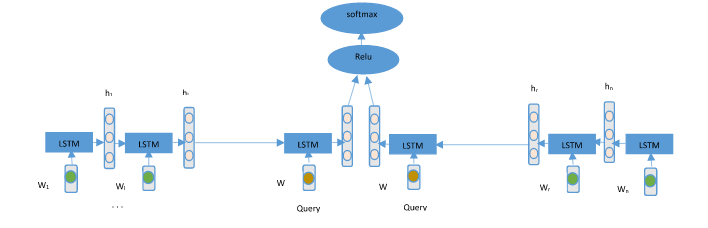
\includegraphics[width=\textwidth]{img/my_model1}
      \caption{Phương pháp sử dụng, . . . . }
       \label{img_my_model1}
\end{figure*}
\par
Mô hình tổng quát được mình họa như hình \ref{img_my_model2}.
\begin{figure*}
     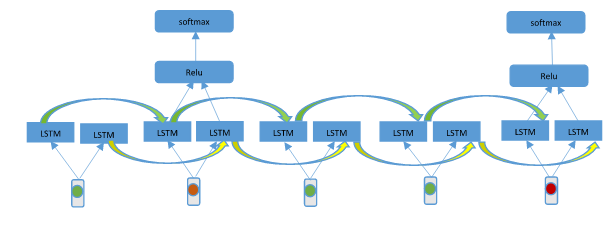
\includegraphics[width=\textwidth]{img/my_model2}
      \caption{Phương pháp sử dụng, . . . . }
       \label{img_my_model2}
\end{figure*}
Trong mô hình sau khi qua mạng LSMT$_{l}$ và LSTM$_{r}$ thì mỗi tầng này sẽ được đưa qua một tầng ẩn với hàm hoạt động là Relu
\begin{center}
$\boldsymbol{out\_relu} = max(0,\boldsymbol{W_{relu}}\cdot [\boldsymbol{h_l},\boldsymbol{h_r}])$\\
\end{center}
Trong đó $W_l$ là ma trận kích thước $H*2H$
Sau đó kết quả đầu ra của tầng Relu sẽ qua một tầng tuyến tính và được tính xác suất cho mỗi lớp dựa trên hàm softmax.\\
\begin{center}
$\boldsymbol{logit} = \boldsymbol{W}\cdot\boldsymbol{out\_relu}$\\
\end{center}
Với $\boldsymbol{W}$ là ma trận KxH, K là số đầu ra mong muốn, H là độ dài của vector ở tầng ẩn của LSTM.\\
Hàm lỗi của mô hình vẫn sẽ là cross-entropy và học dựa trên thuật toán lan truyền ngược [ref] để cập nhập trọng số.
\begin{center}
a
\end{center}
Trong đó S là tập dữ liệu huấn luyện, K là số nhãn, s được hiểu là một truy vấn, $P_c(s)$ là xác suất mô hình dự đoán truy vấn s và lớp c, $P_c^g(s)$ chỉ ra rằng truy vấn s có thuộc lớp c hay không, giá trị của nó nhận là 0 hoặc 1.
\section{Thử nghiệm, đánh giá}\label{sec:exp}
%%%%%%%%%%%%%%%%%%%%%%%%%%%%%%%%%
\subsection{Xây dựng bộ dữ liệu thử nghiệm}
Trên thế giới hiện nay có một số bộ dữ liệu được xây dựng trên ngôn ngữ tiếng anh được thu thập từ twetter như bộ dữ liệu được tác giả Dong giới thiệu trong bài báo  Adaptive recursive neural network for target-dependent twitter sentiment classification \textsuperscript{\cite{dongadaptive}}. Tuy nhiên với tiếng Việt thì hiện tại chưa có bộ dữ liệu nào được tạo ra phục vụ cho bài toán Target-Dependent Sentiment Classification. Do đó để thực hiện thử nghiệm tôi xây dựng một bộ dữ liệu tiếng Việt trên miền dữ liệu nói về xe. Dữ liệu này được thu thập trên các trang báo mạng sau đó được đưa qua bộ tách từ, bộ tách từ tôi xin được phép sử dụng lại từ bộ dữ liệu đã được xây dựng của quý công ty VCcorp Việt Nam. Sau đó dữ liệu được tách thành từng câu và thực hiện gán nhãn quan điểm với 3 nhãn chính là: positive, negative, neutral. Quan điểm của từng từ truy vấn sẽ chỉ phụ thuộc vào phạm vi của câu đang xét.Trong phạm vi miền dữ liệu về xe tôi xin chỉ gán các truy vấn liên quan đến xe.\\
Cùng với đó truy vấn cũng được chia thành hai nhóm trong quá trình gán nhãn là nhóm TERM chỉ những đối tượng và nhóm ASPECT chỉ những khía cạnh, thuộc tính của một đối tượng nào đó. Dưới đây là một vài ví dụ về dữ liệu.\\
\textit{
Ví dụ 1: Gần tết , các đại\_lý " làm\_giá " các mẫu xe " đắt\_khách " của honda{t-negative} như vision{t-negative} , lead{t-negative} , air\_blade{t-negative} , sh\_mode{t-negative} đều bị các đại\_lý " thổi giá{a-negative} \\
Ví dụ 2: Được thành\_lập vào năm 1929 tại đức , borgward{t-negative} đã từng\_trải qua một thời\_gian dài đóng\_cửa vì phá\_sản .
" }
\par
Thống kê số lượng nhãn neutral, positive và negative theo truy vấn được mô tả ở bảng \ref{table:data_des}
\begin{table}[ht]
\begin{center}
  \begin{tabular}{|l|l|l|l|}
\hline
Nhãn & Neutral & Positive & Negative\\
\hline
Số lượng & 43178 & 12567 & 2441\\
\hline
Tỉ lệ & 17.7 & 5.1 & 1\\
\hline
  \end{tabular}
  \end{center}
  \caption{Mô tả thống kê dữ liệu}
  \label{table:data_des}
\end{table}%
\subsection{Các độ đo được sử dụng}
\par
Accuracy: đây là độ đo thông dụng thường được sử dụng trong việc đánh giá các mô hình học máy. Độ đo được tính dựa trên công thức sau:\\
\begin{center}
$Accuracy = \frac{n}{N}$\\
\end{center}
Với n là số nhãn dự đoán đúng và N là tổng số nhãn được dự đoán.
\par
F1: là một độ đo phản ánh trung bình điều hòa giữa hai giá trị precision và recall. Với một bài toán phân loại, precision và recall được tính trên một lớp dựa vào ma trận nhầm lẫn. Với bảng nhầm lẫn được mô tả như bảng \ref{table:con_fus_max}, ta có:\\
\begin{center}
$precision = \frac{TP}{TP+FP}$\\

$recall = \frac{TP}{TP+FN}$\\

$F1 = \frac{2*precision*recall}{precision+recall}$
\end{center}

\begin{table}[ht]
\begin{center}
  \begin{tabular}{|l|l|l|l|}
  \hline
  \multicolumn{2}{|c|}{\multirow{2}{*}{Lớp A}} & 	\multicolumn{2}{|c|}{Mô hình dự đoán}\\ 
  \cline{3-4}
  \multicolumn{2}{|l|}{} & Thuộc A & Không thuộc A  \\
  \cline{1-4}
  \multirow{2}{4em}{Nhãn Đúng} & Thuộc A & TP & FN \\ 
  \cline{2-4}
   & Không thuộc A & FP & TN \\ 
  \hline
  \end{tabular}
  \end{center}
  \caption{Ma trận nhầm lẫn}
  \label{table:con_fus_max}
\end{table}%
%%%%%%%%%%%%%%%%%%%%%%%%%%%%%%%%%%%%%%%%%%
\subsection{Các tham số trong mô hình LSTM}
\par
Dữ liệu sau khi được gán nhãn sẽ được chia thành tập huấn luyện và tập kiểm thử  dựa vào phương pháp Stratified sampling, bằng cách chia ngẫu nhiên mỗi nhãn với tỉ lệ train:test = 3:1.
\subsubsection{Các tham số của mô hình LSTM}\label{set_up_lstm}
\par
Với dữ liệu được mô tả như bảng \ref{table:data_des}, ta thấy rằng dữ liệu thuộc lớp neutral đang quá nhiều, nếu mô hình dự đoán tất cả vào lớp neutral thì độ chính xác accuracy vẫn đạt 74,4\%, đồng thời số lượng dữ liệu positive cũng nhiều hơn đáng kể so với dữ liệu negative. Do đó, để tăng ảnh hưởng của mô hình học đối với lớp dữ liệu negative ta sẽ thực hiện tăng ảnh hưởng của hàm lỗi mỗi khi dự đoán sai đối với nhãn negative, đồng thời giảm ảnh hưởng của hàm lỗi với nhãn positive và neutral. Việc này sẽ tránh mô hình chỉ tập trung vào nhãn có nhiều dữ liệu. Tương ứng với từng nhãn lớp neutral, positive, negative ta sẽ có các trọng số $w_{neutral}$, $w_{positive}$, $w_{negative}$, trong đó $w_{neutral} < w_{positive} < w_{negative}$ thứ tự này được sắp xếp do dữ liệu nhãn neutral nhiều hơn dữ liệu positive và negative, và dữ liệu nhãn positive nhiều hơn dữ liệu nhãn lớp negative. Các trọng số  $w_{neutral}$, $w_{positive}$, $w_{negative}$ là hyparameters nên ta cần lựa chọn trọng số để mô hình học được tốt nhất. Như vậy hàm lỗi sẽ được tính như sau:\\
\begin{center}
$loss = - \sum_{s\in S} \sum_{k=1}^k w_s*P_k^g(s)*log(P_c(s))$\\
\end{center}
Trong đó S là tập dữ liệu huấn luyện, K là số nhãn, s được hiểu là một truy vấn, $P_c(s)$ là xác suất mô hình dự đoán truy vấn s và lớp c, $P_c^g(s)$ chỉ ra rằng truy vấn s có thuộc lớp c hay không, giá trị của nó nhận là 0 hoặc 1, $w_c$ là trọng số lệch nhãn ứng với lớp c.
\par
Không mất tính tổng quát ta hoàn toàn có thể giả sử $w_{neutral}$, $w_{positive}$, $w_{negative}$ thuộc khoảng [0,1] và $w_{negative}$ sẽ được cố định bằng 1.
Đặt:\\
\begin{center}
$w'_{neutral} = \frac{w_{neutral}}{w_{negative}}$\\
$w'_{positive} = \frac{w_{positive}}{w_{negative}}$\\
$w'_{negative} = 1$\\
\end{center}
Khi đó hàm lỗi sẽ được viết lại thành:\\
\begin{center}
$loss = - w_{negative}*\sum_{s\in S} \sum_{k=1}^k w'_s*P_k^g(s)*log(P_c(s))$\\
\end{center}
Do $w_{negative}$ là hằng số nên việc bỏ đi $w_{negative}$ sẽ không ảnh hưởng đến giá trị tối ưu của hàm số.
\par
Dựa trên tỉ lệ nhãn từ bảng \ref{table:data_des}, giá trị của $w_{neutral}$ sẽ thay đổi quanh giá trị $\frac{1}{17.7} \approx 0.06  $, $w_{positive}$ sẽ thay đổi quan giá trị $\frac{1}{5.1} \approx 0.2$ và $w_{negative}$ sẽ được cố định là 1.
\par
Các tham số cài đặt của mô hình LSTM được mô tả như sau
\begin{itemize}
\item batch size: số lượng dữ liệu được đưa vào mỗi lượt lần truyền tiến và lan truyền ngược tỏng mạng nhân tạo, trong đồ án tôi sẽ thử nghiệm hai giá trị là 50 và 100
\item length sentence: độ dài tối đa cho một câu là 70, nếu quá 70 từ thì mô hình sẽ tự động cắt bỏ phần dư thừa
\item LSTM layer: số tầng LSTM sử dụng cho bài toán
\item learning rate: $10^{-3}$ và sử dụng phương pháp cập nhập adam [ref]
\item imbalance weight: trọng số lệch nhãn đối với $w_{neutral}$ sẽ thuộc tập các giá trị [0.03, 0.06, 0.09], trọng số lệch nhãn đối với $w_{positive}$ sẽ thuộc tập các gía trị [0.1, 0.2, 0.3] với $w_{negative}$ được cố định là 1.
\item epoch: số lần toàn bộ dữ liệu được đưa vào huấn luyện, trong đồ án giá trị epoch tối đa sẽ là 65
\item initialization method: khởi tạo các bộ trọng số sử dụng khởi tạo ngẫu nhiên, với phân phối chuẩn (normal distribution) có kì vọng là 0 và độ lệch chuẩn là 1
\item dropout: sử dụng các giá trị dropout với tầng input và tầng relu với giá trị lần lượt là 0.2 và 0.5
\end{itemize}
\subsection{Xét ảnh hưởng của tham số và lựa chọn tham số dựa trên tập validation}
Trong phần này tôi sẽ sử dụng tập validation để thực hiện lựa chọn các tham số tốt nhất đối với mô hình đã đề xuất phía trên. Trong mô hình có ba tham số chính là \textit{batch size}, \textit{imbalance weight} và \textit{epoch}. Trong các phần phía dưới sẽ lần lượt thực hiện xét ảnh hưởng của tham số \textit{batch size}, \textit{imbalance weight}, mỗi trường hợp sẽ thử nghiệm với số lượng epoch cố định là 65 epoch và thực hiện đánh giá trên bộ validation sau mỗi 5 epoch.
\subsubsection{Xét ảnh hưởng tham số lệch nhãn}
Tham số lệch nhãn thay đổi sẽ làm thay đổi mức độ quan trọng của các nhãn trong hàm lỗi. Dựa trên tỉ lệ của nhãn ta có bộ tham số ứng với tỉ lệ nhãn là [0.06,0.2,1], vì lý do đó, bộ lệch nhãn này sẽ được coi là bộ lệch nhãn chuẩn để so sánh các trường hợp. Sau đây sẽ xét ảnh hưởng của tham số lệch nhãn xoay quanh bộ tham số chuẩn [0.06,0.2,1]
\paragraph*{Giữ nguyên trọng số $w_{positive}$ và thay đổi trọng số của $w_{neutral}$}:\\
Trọng số của $w_{neutral}$ được thử nghiệm với các giá trị 0.03, 0.06 và 0.09. Như kết quả được mô tả trong hình vẽ \ref{w_neutral}, khi thay đổi
\begin{figure*}
     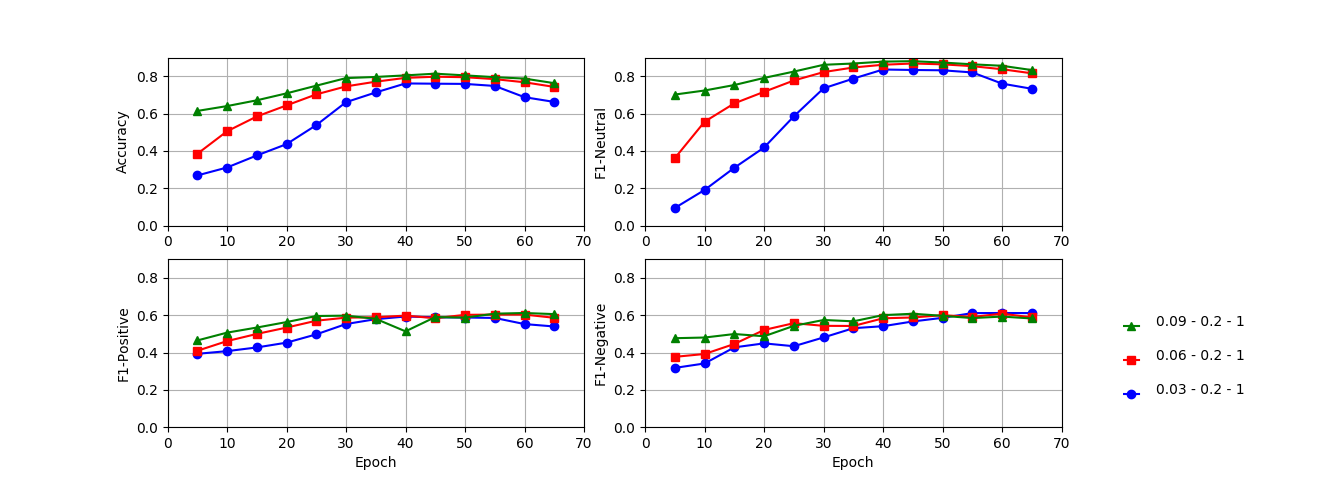
\includegraphics[width=\textwidth]{img/so_sanh_1}
      \caption{Thay đổi trọng số $w_{neutral}$}
       \label{w_neutral}
\end{figure*}
\paragraph*{Giữ nguyên trọng số $w_{neutral}$ và thay đổi trọng số của $w_{positive}$}
\paragraph*{Đồng thời tăng hoặc giảm trọng số  \boldsymbol{$w_{neutral}$} và $w_{positive}$}
\paragraph*{Tăng trọng số $w_{neutral}$ và giảm trọng số \boldsymbol{$w_{positive}$}}
\paragraph*{Tăng trọng số $w_{positive}$ và giảm trọng số \boldsymbol{$w_{neutral}$}}
\paragraph*{Không sử dụng trọng số lệch nhãn và sử dụng trọng số lệch nhãn chuẩn}

\subsubsection{Xét ảnh hướng tham số batch size}
Để xét ảnh hưởng của tham số \textit{batch size} ta lựa ngẫu nhiên một vài trường hợp \textit{imbalance weight} sau đó thực hiện đánh giá để tìm ra \textit{batch size} phù hợp và ổn định nhất.
Dưới đây là 4 bộ tham số ngẫu nhiên dược
\subsection{So sánh phương pháp sử dụng với phương pháp SVM và KNN}
\par
Để so sánh hiệu quả của phương pháp, tôi xin so sánh kết quả tốt nhất phương pháp thu được với các phương pháp SVM và KNN.
\par
Hai phương pháp này được cài đặt dựa trên biểu diễn Tf-idf. Tuy nhiên như đã phân tích ở trên thì các từ truy vấn sẽ có rất nhiều trường hợp là các danh từ riêng nên để giảm chiều của tập từ điển và có biểu diễn hiệu quả hơn thì các từ truy vấn sẽ được chuyển về các nhóm cụ thể. Với giả thiết đầu vào của mô hình sẽ biết truy vấn nào là TERM và truy vấn nào là ASPECT.
\par
Với những truy vấn thuộc nhóm TERM thì từ truy vấn sẽ được thay thế hết bởi từ TERM. Với những truy vấn thuộc nhóm ASPECT, dựa trên tập dữ liệu huấn luyện, các truy vấn thuộc nhóm ASPECT sẽ được lọc ra và phân vào các nhóm:
\begin{itemize}
\item Nhóm công nghệ: những từ chỉ những công nghệ trong miền xe sẽ được đưa vào nhóm này, ví dụ như: \textit{công nghệ camera lùi, công nghệ giảm ma sát}
\item Nhóm dịch vụ: những từ chỉ những dịch vụ liên quan trong miền xe, ví dụ như: \textit{dịch vụ hậu mãi, gói bảo hiểm}
\item Nhóm doanh sô: những từ chỉ doanh số của hãng xe hay doanh số một dòng xe thu được. ví dụ như: \textit{doanh thu, lợi nhuận, doanh số}
\item Nhóm chỉ giá: nhóm nhứng từ nói về giá sảm phẩm, giá chung của một hãng xe, ví dụ như: \textit{giá thành, giá}
\item Nhóm hệ thống: nhóm những từ chỉ những hệ thống trong xe như: \textit{hệ thống định vị, hệ thống truyền lực}
\item Nhóm hiệu năng: nhóm những từ chỉ hiệu năng của một sản phẩm hay hiệu năng chung của một hãng xe, ví dụ như: \textit{công suất, hiệu năng}
\item Nhóm khối lượng: những từ chỉ khối lượng, trọng lượng của xe, ví dụ như: \textit{khối lượng, trọng lượng}
\item Nhóm nhiên liệu: nhóm từ này nói về mức tiêu hao nhiên liệu và lượng khí thải, ví dụ như: \textit{lượng tiêu thụ nhiên liệu, mức khí thải}
\item Nhóm nội ngoại thất: nhóm chỉ các thành phần nội và ngoại thất của xe như: \textit{xi nhan, ghế ngồi}
\item Nhóm ngoại hình: nhóm chỉ thiết kế, ngoại hình và hình dáng, ví dụ như: \textit{thiết kế thân xe, vẻ ngoài}
\item Nhóm thương hiệu: những từ nói về thương hiệu của hãng xe hay sản phẩm như: \textit{thương hiệu, nhãn hiệu}
\item Nhóm other: nhóm này chưa những từ không có trong các nhóm trên, đặc biệt được dùng nhiều cho bộ TEST
\end{itemize}
\par
Quá trình phân nhóm các truy vấn thuộc nhóm ASPECT được thực hiện bằng tay và một phần dựa trên khoảng cách Levenshtein, một khoảng cách sử dụng trong xâu kí tự. Tất cả các từ trong một nhóm sẽ được thay thế chung bởi tên nhóm đó. Trong quá trình đánh giá trên bộ test thì những truy vấn thuộc nhóm ASPECT không có trong nhóm nào sẽ được coi là thuộc nhóm \textit{other}.
\par
Sau bước giảm chiều từ điển trên, mỗi một từ đích sẽ được biểu diễn dựa trên w-s từ bên trái và w-s từ bên phải, w-s này được gọi là window-size, w-s sẽ được thay đổi với các giá trị 5, 9, 15, 30. Gọi mỗi biểu diễn là \textit{văn bản truy vấn}
\par
Các văn bản truy vấn từ bộ dữ liệu huấn luyện sẽ được biểu diễn dưới dạng vector tf-idf và đồng thời tính trọng số idf và tạo ra bộ từ điển dựa trên bộ dữ liệu huấn luyện. Trong bài tóan này tôi không lọc bỏ từ dừng và lấy toàn bộ từ trong tập từ điển.
\par
Dựa vào trọng số idf từ bộ dữ liệu huấn luyện và tập từ điển, mỗi văn bản truy vấn trong bộ kiểm thử cũng sẽ được biểu diễn dưới dạng tf-idf.
\par
Mô tả các tham số trong mô hình học KNN và SVM
\begin{itemize}
\item SVM: mô hình sẽ sử dụng hàm kernel là linear và do dữ liệu lệch nhãn nên sử dụng thêm bộ trọng số cho bài toán lệch nhãn, với những bộ thử nghiệm giống như sử dụng với mô hình LSTM mục \ref{set_up_lstm} 
\item KNN: ngoài tham số là window-size thì số lượng hàng xóm k, trong bài toán k = [5, 15, 30]
\end{itemize}
\par
Bảng \ref{table:compare_lstm} mô tả so sánh về độ chính xác và các độ đo F1 đối với các nhãn neutral, positive, negative. Trong bảng so sánh các mô hình đều được thực hiện việc chọn tham số tốt nhất dựa vào tập validation sau đó sử dụng bộ tham số này và học lại trên toàn bộ tập train và validation sau đó đánh giá trên tập test.
\par
Ta thấy rằng mô hình KNN mặc dù có giá trị Accuracy cao nhưng khi xem xét về độ đo F1-Neutral, F1-Positive, F1-Negative thì ta thấy rằng mô hình này không thực sự hoạt động tốt với bài toán lệch nhãn và mô hình dự đoán hầu hết vào lớp Neutral.
\par
Bên cạnh đó SVM đạt được kết quả rất khả quan với độ chính xác thấp hơn so với mô hình KNN Nhưng trái lại SVM có độ F1-Neutral, F1-Positive, F1-Negative cao hơn và đương đầu với bài toán lệch nhãn tốt khi ta sử dụng thêm trọng số lệch nhãn 
\begin{table}[ht]
\begin{center}
  \begin{tabular}{|l|l|l|l|l|}
  \hline
  Phương pháp & Accuracy & F1-Neutral & F1-Positive & F1-Negative\\
  \hline
  K-NN & 77.5 & 86 & 41.5 & 41.7\\
  \hline
  $SVM^*$ & 76.9 & 85.5 & 46.4 & 40.7\\
  \hline
  SVM & 73 & 81.6 & 52.8 & 50.9\\
  \hline
  $LSTM^*$ & 80 & 86 & 61.4 & 58.7\\
  \hline
  LSTM & 77 & 86 & 60 & 60\\
  \hline
  \end{tabular}
  \end{center}
  \caption{Bảng so sánh độ chính xác accuracy và giá trị f1 qua tác nhãn neutral, positive, negative. Dấu * thể hiện mô hình không sử dụng trọng số lệch nhãn}
  \label{table:compare_lstm}
\end{table}%
\newpage
%%%%%%%%%%%%%%%%%%%%%%%%%%%%%%%%%%%%%%%%%%%%%%%%%%%%%%%%%%%%%%%%%%
\section{Kết luận}\label{sec:end}
Tổng kết lại đồ án

\newpage
\bibliographystyle{plain}
\bibliography{ref}
\end{document}
